%
% normalverteilung.tex -- Abschnitt ueber Normalverteilung in Kapitel 5
%
% (c) 2015 Prof Dr Andreas Mueller, Hochschule Rapperswil
%
\subsection{Normalverteilung} \label{normalverteilung}
\index{Normalverteilung}
\begin{table}
\renewcommand{\arraystretch}{2}
\begin{center}
\begin{tabular}{|l|l|}
\hline
Name&Normalverteilung\\
\hline
\setlength{\extrarowheight}{2pt}
Dichtefunktion&$\displaystyle\frac{1}{\sqrt{2\pi}\sigma}e^{-\frac{(x-\mu)^2}{2\sigma^2}}$\\
Verteilungsfunktion&keine elementare Funktion\\
Erwartungswert&$\mu$\\
Varianz&$\sigma^2$\\
Median&$\mu$\\
$P(|X-E(X)|>\varepsilon)$&keine einfache Formel\\
\hline
%\setlength{\extrarowheight}{50pt}
Anwendungen&
\begin{minipage}{3.7in}%
\vskip4pt
\strut
$\bullet$ Messwerte\\
$\bullet$ Summe vieler kleiner Einflüsse vergleichbar grosser Varianz
(Zentraler Grenzwertsatz)
\\
$\bullet$ Approximation der Binomialverteilung
\strut
\end{minipage}\\[21pt]
\hline
\end{tabular}
\end{center}
\caption{Datenblatt der Normalverteilung\label{datenblatt:normalverteilung}}
\end{table}
\begin{figure}
\begin{center}
%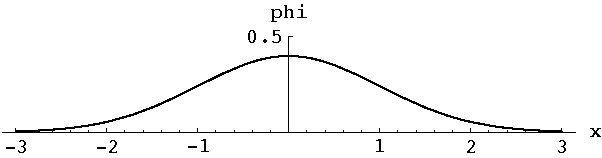
\includegraphics[width=0.8\hsize]{graphics/normphi}
%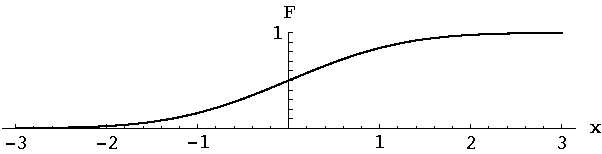
\includegraphics[width=0.8\hsize]{graphics/normF}
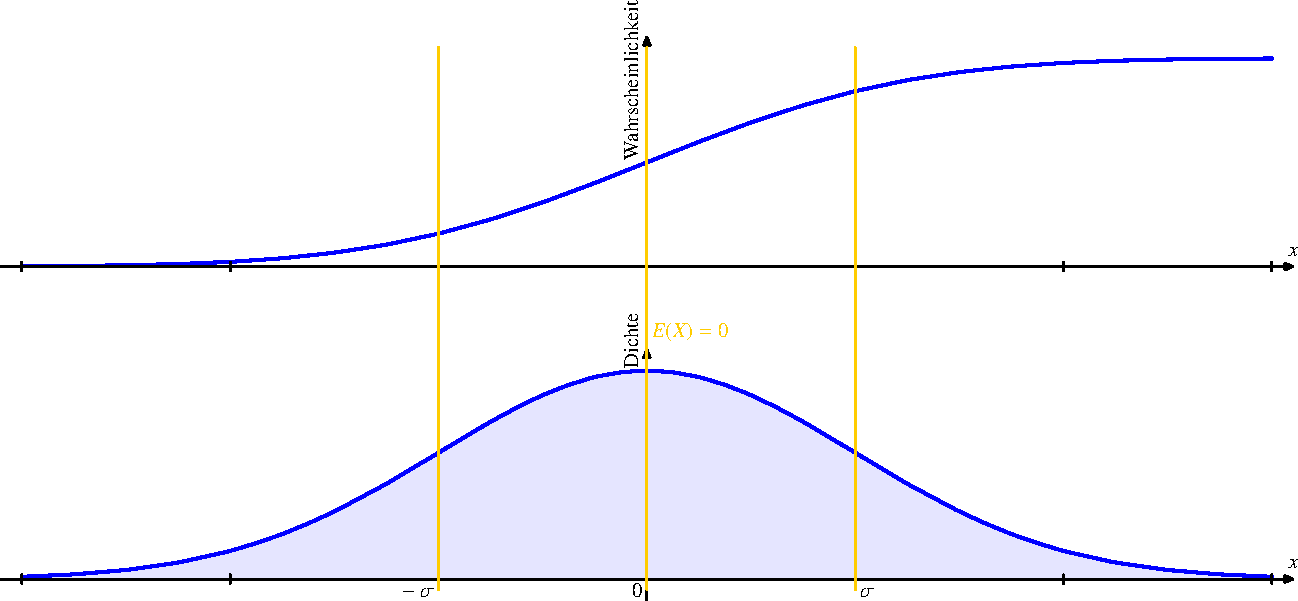
\includegraphics[width=\hsize]{images/verteilungsfunktion-9}
\end{center}
\caption{Verteilungsfunktion (oben) und Dichtefunktion (unten) der Normalverteilung\label{bildnormalverteilung}}
\end{figure}
Die Normalverteilung, auch Gaussverteilung genannt, ist von grosser praktischer
Bedeutung.
In sehr vielen Anwendungssituationen darf man davon ausgehen,
dass die beobachteten Zufallsgrössen normalverteilt sind.
Die Begründung
für diesen überraschenden Sachverhalt liefert der Zentrale Grenzwertsatz,
welcher im wesentlich besagt, dass eine Zufallsvariable, die als Summe vieler
kleiner, unabhängiger Zufallseinflüsse betrachtet werden kann, immer
angenähert normalverteilt ist.
Wir werden diesen Sachverhalt ab Seite \pageref{zentraler-grenzwertsatz}
und in Satz~\ref{satz-zentraler-grenzwertsatz} genauer formulieren.

\subsubsection{Dichtefunktion, Erwartungswert und Varianz}
\index{Wahrscheinlichkeitsdichte!der Normalverteilung}
\index{Normalverteilung!Wahrscheinlichkeitsdichte}
\begin{definition}
Eine Zufallsvariable $X$ heisst normalverteilt mit Erwartungswert $\mu$ und
Varianz $\sigma^2$, wenn sie die
Dichtefunktion
\[
\varphi(x)=\frac1{\sigma\sqrt{2\pi}}e^{-\frac{1}{2}
\left(\frac{x-\mu}{\sigma}\right)^2}
\]
hat.
\end{definition}
\index{Standardnormalverteilung}%
\index{Normalverteilung!Standard-}%
Die Verteilungsfunktion der Normalverteilung mit Erwartungswert $0$
und Varianz $1$, der sogenannten Standardnormalverteilung, kann nicht in
geschlossener Form gefunden werden, es müssen entweder Tabellen
oder numerische Lösungen verwendet werden.

Die Werte der Verteilungsfunktion der Standardnormalverteilung sind 
tabelliert, zum Beispiel auch in Tabelle~\ref{tabelle-Fnormalverteilung}.
Daraus kann man zum Beispiel die folgenden Werte ablesen
\begin{align*}
F(1)&=0.8413,&F(-1)&=1-F(1)=0.1587&&\Rightarrow&P(-1<X\le 1)&=68.28\%\\
F(2)&=0.9772,&F(-2)&=1-F(2)=0.0228&&\Rightarrow&P(-2<X\le 2)&=95.4\%\\
F(3)&=0.9987,&F(-3)&=1-F(3)=0.0013&&\Rightarrow&P(-3<X\le 3)&=99.7\%
\end{align*}
Zwei Drittel aller Messwerte fallen also in das Intervall $[-1,1]$, und 95\%
aller Messwerte in das Intervall $[-2,2]$.

Man kann die Verteilungsfunktion der Standardnormalverteilung auch wie folgt
numerisch zu berechnen versuchen:
\begin{equation}
\begin{aligned}
P(X\le x)
&=\frac1{\sqrt{2\pi}}\int_{-\infty}^xe^{-\frac12\xi^2}\,d\xi\\
&=\frac12+\frac1{\sqrt{2\pi}}\int_0^xe^{-\frac12\xi^2}\,d\xi\\
&=\frac12+\frac1{\sqrt{\pi}}\int_0^xe^{-\frac12\xi^2}\,\frac{d\xi}{\sqrt{2}}\\
&=\frac12+\frac1{\sqrt{\pi}}\int_0^{\frac{x}{\sqrt{2}}}e^{-t^2}\,dt\\
\end{aligned}
\label{normal-werte}
\end{equation}
Der zweite Term kann mit Hilfe der Fehlerfunktion 
\[
\operatorname{erf}(x)=\frac{2}{\sqrt{\pi}}\int_0^xe^{-t^2}\,dt
\]
umgeformt werden:
\begin{equation}
P(X\le x)=\frac12\biggl(1+\operatorname{erf}\biggl(\frac{x}{\sqrt{2}}\biggr)\biggr).
\label{Fnormal-erf}
\end{equation}
\index{Fehlerfunktion}%
\index{Verteilungsfunktion!Normalverteilung}%
Die Fehlerfunktion ist eine ungerade Funktion mit Wertebereich $(-1,1)$,
sie ist in vielen Softwaresystemen als Bibliotheksfunktion verfügbar, in
der C-Bibliothek steht zum Beispiel neben $\operatorname{erf}(x)$ auch
$1-\operatorname{erf}(x)$ zur Verfügung.
Da $\lim_{x\to\infty}\operatorname{erf}(x)=1$ könnten Werte von
$1-\operatorname{erf}(x)$ für grosse Werte von $x$ nur mit grossen Fehlern 
berechnet werden, die komplementäre Fehlerfunktion löst dieses Problem.

Für eine normalverteilte Zufallsvariable $X$ mit Erwartungswert $\mu$ und
Standardabweichung $\sigma$ ist die Tabelle oder die Formel (\ref{Fnormal-erf})
nicht anwendbar. 
Man kann jedoch mit der Standardisierung aus Abschnitt~\ref{section-standardisierung}
immer zu einer Zufallsvariable $Z=(X-\mu)/\sigma$ gelangen, die
standardnormalverteilt ist.
Damit lässt sich auch die Wahrscheinlichkeit ermitteln:
\begin{align*}
P(a<X\le b)
&=
P\biggl(\frac{a-\mu}{\sigma}<\frac{X-\mu}{\sigma}\le \frac{b-\mu}{\sigma}\biggr)
=
F\biggl(\frac{b-\mu}{\sigma}\biggr)
-
F\biggl(\frac{a-\mu}{\sigma}\biggr).
\end{align*}
Die Werte von $F$ können entweder der Tabelle~\ref{tabelle-Fnormalverteilung}
entnommen oder mit der Formel (\ref{Fnormal-erf}) berechnet werden.
Die Werte in (\ref{normal-werte}) bedeuten dann, dass gut zwei Drittel aller
Messwerte in das Intervall $[\mu-\sigma, \mu+\sigma]$ fallen, und dass 
95\% der Messwerte sich in $[\mu-2\sigma,\mu+2\sigma]$ befinden.

Der Vollständigkeit halber rechnen wir nach, ob die durch $\varphi$
definierte Verteilung tatsächlich die behaupteten Eigenschaften hat.
Zunächst hat man die allgemeine Formel:
\begin{align*}
\int_{-\infty}^{\infty}f(x)\varphi(x)\,dx
&=\frac1{\sigma\sqrt{2\pi}}\int_{-\infty}^{\infty}f(x)e^{-\frac{1}{2}\left(\frac{x-\mu}{\sigma}\right)^2}\,dx\\
&=\frac1{\sqrt{2\pi}}\int_{-\infty}^{\infty}f(\sigma\xi+\mu)e^{-\frac{\xi^2}2}\,d\xi
\end{align*}
Daraus kann man jetzt den Erwartungswert bestimmen indem man $f(x)=x$ verwendet:
\begin{align*}
E(X)
&=\frac1{\sqrt{2\pi}}\int_{-\infty}^{\infty}(\sigma\xi+\mu)e^{-\frac{\xi^2}2}\,d\xi\\
&=\sigma\frac1{\sqrt{2\pi}}\int_{-\infty}^{\infty}\xi e^{-\frac{\xi^2}2}\,d\xi+
\mu\frac1{\sqrt{2\pi}}\int_{-\infty}^{\infty}e^{-\frac{\xi^2}2}\,d\xi
\end{align*}
Für das erste Integral benutzt man
\[
\frac{d}{d\xi}e^{-\frac{\xi^2}{2}}=-\xi e^{-\frac{\xi^2}{2}}
\]
woraus folgt
\[
\frac1{\sqrt{2\pi}}\int_{-\infty}^{\infty}\xi e^{-\frac{\xi^2}2}\,d\xi
=
-\frac1{\sqrt{2\pi}}\left[
 e^{-\frac{\xi^2}2}
\right]_{-\infty}^{\infty}=0
\]
Um das zweite Integral benutzt man wir den Trick, dass wir dessen
Quadrat bestimmen:
\begin{align*}
\biggl(\frac{1}{\sqrt{2\pi}}\int_{-\infty}^{\infty}e^{-\frac{x^2}2}\,dx\biggr)^2
&=
\frac1{\sqrt{2\pi}}\int_{-\infty}^{\infty} e^{-\frac{\xi^2}2}\,d\xi\cdot
\frac1{\sqrt{2\pi}}\int_{-\infty}^{\infty} e^{-\frac{\eta^2}2}\,d\eta\\
&=
\frac1{2\pi}\int_{-\infty}^{\infty}\int_{-\infty}^{\infty}
e^{-\frac{\xi^2+\eta^2}2}
\,d\xi\,d\eta\\
&=
\frac1{2\pi}\int_{0}^{\infty}\int_{0}^{2\pi}re^{-\frac{r^2}2}\,d\varphi\,dr\\
&=\int_0^{\infty}re^{-\frac{r^2}2}\,dr
=\bigl[-e^{-\frac{r^2}2}\bigr]_0^{\infty}
=1
\end{align*}
Dabei haben wir in der dritten Zeile auf Polarkoordinaten gewechselt.
Somit ist $E(X)=\mu$.

\index{Erwartungswert!Normalverteilung}
\index{Normalverteilung!Erwartungswert}
\index{Varianz!Normalverteilung}
\index{Normalverteilung!Varianz}
Für die Varianz von $(x-\mu)$ können wir annehmen, dass $\mu=0$, dann
genügt es, $E(X^2)$ zu berechnen:
\begin{align*}
E(X^2)
&=\frac1{\sqrt{2\pi}}\int_{-\infty}^{\infty}(\sigma\xi)^2e^{-\frac{\xi^2}2}\,d\xi\\
&=\sigma^2\frac{1}{\sqrt{2\pi}}\int_{-\infty}^{\infty}\xi^2e^{-\frac{\xi^2}2}\,d\xi
\end{align*}
Das Integral kann durch partielle Integration mit den Faktoren
$\xi$ und $\xi e^{-\frac{\xi^2}2}$ vereinfacht werden:
\begin{align*}
E(X^2)
&=\sigma^2\frac{1}{\sqrt{2\pi}}\int_{-\infty}^{\infty}\xi^2e^{-\frac{\xi^2}2}\,d\xi\\
&=\sigma^2\frac{1}{\sqrt{2\pi}}\biggl(
\biggl[\xi e^{-\frac{\xi^2}2}\biggr]_{-\infty}^{\infty}
+
\int_{-\infty}^{\infty}e^{-\frac{\xi^2}2}\,d\xi
\biggr)\\
&=\sigma^2\frac{1}{\sqrt{2\pi}}
\int_{-\infty}^{\infty}e^{-\frac{\xi^2}2}\,d\xi\\
&=\sigma^2
\end{align*}
Also ist $\operatorname{var}(X)=\sigma$.

Integrale von Ausdrücken der Form
$e^{-\frac12(ax^2+bx+c)}$
kommen beim Rechnen mit der Normalverteilung immer wieder vor, deshalb
stellen wir das Resultat in Form eines Hilfssatzes bereit:
\begin{hilfssatz}
\label{exp-quadr}
Ist $a>0$, dann gilt
\[
\frac1{\sqrt{2\pi}}\int_{-\infty}^{\infty}\exp\left(-\frac12(ax^2+bx+c)\right)\,dx
=
\frac1{\sqrt{a}}\exp\left(-\frac12\left(c-\frac{b^2}{4a}\right)\right).
\]
\end{hilfssatz}
\begin{proof}[Beweis]
Durch quadratisches Ergänzen kann man den Ausdruck $ax^2+bx+c$ umschreiben in
\[
ax^2+bx+c=a\left(x-\frac{b}{2a}\right)^2+c-\frac{b^2}{4a}.
\]
Damit lässt sich das Integral wie folgt vereinfachen:
\begin{align*}
&\phantom{=}\frac1{\sqrt{2\pi}}\int_{-\infty}^{\infty}\exp\biggl(-\frac12\biggl(
a\biggl(x-\frac{b}{2a}\biggr)^2+c-\frac{b^2}{4a}
\biggr)\biggr)\,dx\\
&=\frac1{\sqrt{2\pi}}
\exp\biggl(-\frac12\biggl(
c-\frac{b^2}{4a}
\biggr)\biggr)
\int_{-\infty}^{\infty}
\exp\biggl(-\frac12\biggl(
a\biggl(x-\frac{b}{2a}\biggr)^2
\biggr)\biggr)
\,dx\\
&=
\exp\biggl(-\frac12\biggl(
c-\frac{b^2}{4a}
\biggr)\biggr)
\frac1{\sqrt{2\pi}}
\int_{-\infty}^{\infty}
\exp\left(-\frac12
a\xi^2
\right)
\,d\xi\\
&=
\exp\biggl(-\frac12\biggl(
c-\frac{b^2}{4a}
\biggr)\biggr)
\frac1{\sqrt{2\pi}}
\int_{-\infty}^{\infty}
\exp\left(-\frac12
\eta^2
\right)
\,\frac{d\eta}{\sqrt{a}}\\
&=
\frac{1}{\sqrt{a}}
\exp\biggl(-\frac12\biggl(
c-\frac{b^2}{4a}
\biggr)\biggr)
\end{align*}
Wobei wir in der dritten Zeile die Substitution $\xi=x-\frac{b}{2a}$
und in der vierten die Substitution
$\eta=\sqrt{a}\xi$
verwendet haben.
\end{proof}

\subsubsection{Summe normalverteilter Zufallsvariablen}
\index{Summe normalverteilter Zufallsvariablen}
\index{Faltung der Normalverteilung}

Eine besonders wichtige Eigenschaft der Normalverteilung ist, dass die
Summe zweier unabhängiger normalverteilter Zufallsgrössen wieder normalverteilt
ist.
\begin{satz}
Sind $X_1$ und $X_2$ normalverteilte Zufallsgrössen mit Mittelwert $\mu_1$
resp.~$\mu_2$ und Varianz $\sigma_1$ resp.~$\sigma_2$, dann ist
$X_1+X_2$ ebenfalls normalverteilt mit Mittelwert $\mu_1+\mu_2$ und
Varianz $\sigma^2=\sigma_1^2+\sigma_2^2$.
\end{satz}
\begin{proof}[Beweis]
Aus der Linearität des Erwartungswertes ist klar, dass der Mittelwert
$\mu=\mu_1+\mu_2$ sein muss.
Auch wissen wir bereits aus Satz \ref{rechenregeln-varianz}, dass
die Varianz der Summe $X_1+X_2$ die angegebene Form hat.
Es ist also nur
noch nachzuprüfen, dass die Dichtefunktion wieder die eine Normalverteilung
ist.

Zunächst haben offensichtlich $X_1$ und $X_1-\mu_1$ Dichtefunktionen,
die sich nur durch eine Translation um $\mu_1$  unterscheiden, ebenso
$X_2$ und $X_1+X_2$.
Es genügt also, den Fall $\mu_1=\mu_2=0$ zu untersuchen.

Wir berechnen die Dichtefunktion der Verteilung der Summe $X=X_1+X_2$
mit Hilfe der Faltung. 
Dazu muss das Integral 
\begin{align*}
\varphi_1*\varphi_2(z)
&=
\int_{-\infty}^{\infty}\varphi_1(t)\varphi_2(z-t)\,dt\\
&=
\int_{-\infty}^{\infty}
\frac1{\sigma_1\sqrt{2\pi}}e^{-\frac12\left(\frac{t}{\sigma_1}\right)^2}
\frac1{\sigma_2\sqrt{2\pi}}e^{-\frac12\left(\frac{z-t}{\sigma_2}\right)^2}
\,dt\\
&=
\frac1{\sigma_1\sqrt{2\pi}}
\frac1{\sigma_2\sqrt{2\pi}}
\int_{-\infty}^{\infty}
e^{-\frac12\left(\frac{t}{\sigma_1}\right)^2}
e^{-\frac12\left(\frac{z-t}{\sigma_2}\right)^2}
\,dt\\
&=
\frac1{\sigma_1\sqrt{2\pi}}
\frac1{\sigma_2\sqrt{2\pi}}
\int_{-\infty}^{\infty}
\exp\biggl(-\frac12\biggl[\biggl(\frac{t}{\sigma_1}\biggr)^2
+\left(\frac{z-t}{\sigma_2}\right)^2\biggr]\biggr)
\,dt
\end{align*}
ausgewertet werden.
Im Exponenten in der eckigen Klammer steht der Ausdruck
\[
\biggl(\frac{t}{\sigma_1}\biggr)^2 +\left(\frac{z-t}{\sigma_2}\right)^2,
\]
den wir durch Ausmultiplizieren in die Form
\[
\biggl(\frac1{\sigma_1^2}+\frac1{\sigma_2^2}\biggr)t^2
-\frac{2z}{\sigma_2^2}t+\frac{z^2}{\sigma_2^2}
\]
bringen können.
Das ist genau die Form, für das im Hilfssatz \ref{exp-quadr}
ein Resultat bereitgestellt wurde, wobei jetzt folgende Werte für $a$, $b$ und $c$
zu verwenden sind:
\[
a=\left(\frac1{\sigma_1^2}+\frac1{\sigma_2^2}\right)
=\frac{\sigma_1^2+\sigma_2^2}{\sigma_1^2\sigma_2^2},\qquad
b=\frac{2z}{\sigma_2^2},\qquad
c=\frac{z^2}{\sigma_2^2}
\]
Setzt man diese Werte in das Resultat von Hilfssatz \ref{exp-quadr} ein,
ergibt sich
\begin{align*}
\varphi_1*\varphi_2(z)
&=
\frac1{\sigma_1\sqrt{2\pi}}
\frac1{\sigma_2\sqrt{2\pi}}
\int_{-\infty}^{\infty}
\exp\biggl(-\frac12\biggl[\biggl(\frac{t}{\sigma_1}\biggr)^2
+\left(\frac{z-t}{\sigma_2}\right)^2\biggr]\biggr)
\,dt\\
&=
\frac1{\sqrt{\sigma_1^2+\sigma_2^2}\sqrt{2\pi}}
\exp\biggl(-\frac12\biggl[c-\frac{b^2}{4a} \biggr]\biggr)
\end{align*}
Der Ausdruck in der eckigen Klammer wird zu
\begin{align*}
c-\frac{b^2}{4a}
&=
\frac{z^2}{\sigma_2^2}
-
\frac{4z^2}{\sigma_2^4}
\frac{\sigma_1^2\sigma_2^2}{\sigma_1^2+\sigma_2^2}
\frac14\\
&=
\frac{z^2}{\sigma_2^2}
-
\frac{z^2}{\sigma_2^2}
\frac{\sigma_1^2}{\sigma_1^2+\sigma_2^2}
=
\frac{z^2}{\sigma_2^2}
\left(
1-\frac{\sigma_1^2}{\sigma_1^2+\sigma_2^2}
\right)\\
&=
\frac{z^2}{\sigma_2^2}
\frac{\sigma_2^2}{\sigma_1^2+\sigma_2^2}
=
\frac{z^2}
{\sigma_1^2+\sigma_2^2}
\end{align*}
Woraus sich für das Faltungsprodukt
\begin{align*}
\varphi_1*\varphi_2(z)
&=
\frac1{\sqrt{\sigma_1^2+\sigma_2^2}\sqrt{2\pi}}
\exp\biggl(-\frac12\frac{z^2}{\sigma_1^2+\sigma_2^2}\biggr)
\end{align*}
ergibt, was genau die Wahrscheinlichkeitsdichte der Normalverteilung
mit Varianz $\sqrt{\sigma_1^2+\sigma_2^2}$ darstellt.
\end{proof}

\subsubsection{Wahrscheinlichkeit grosser Abweichungen}
\begin{figure}
\begin{center}
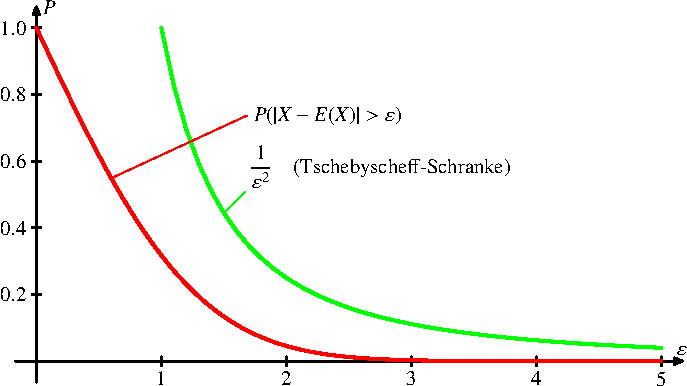
\includegraphics{images/norm-1.pdf}
\end{center}
\caption{Vergleich der Wahrscheinlichkeit für eine grosse Abweichung
für die Normalverteilung (rot) und die Schranke von Tschebyscheff (grün)
\label{abweichung-normalverteilung}}
\end{figure}

Auch für die Normalverteilung wollen wir die Wahrscheinlichkeit
für grosse Abweichungen berechnen.
Es gilt wieder
\[
P(|X-\mu|>\varepsilon)
=1-\int_{-\varepsilon}^{\varepsilon}e^{-\frac{x^2}{2\sigma^2}}\,dx
=
1-{\textstyle\frac12}(\operatorname{erf}({\textstyle\frac{\varepsilon}{\sigma\sqrt{2}}})-\operatorname{erf}({\textstyle-\frac{\varepsilon}{\sigma\sqrt{2}}}))
=
1-\operatorname{erf}({\textstyle\frac{\varepsilon}{\sigma\sqrt{2}}})
\]
Die Abbildung~\ref{abweichung-normalverteilung} zeigt die Wahrscheinlichkeit
für eine grosse Abweichung vom Mittelwert ein Einheiten
von $\sqrt{\operatorname{var}(X)}$.
Noch deutlicher als bei der
Exponentialverteilung zeigt sich, dass die zusätzliche Information
über die Verteilung die Wahrscheinlichkeit für eine grosse
Abweichung deutlich besser abschätzen lässt.

\subsubsection{Der zentrale Grenzwertsatz}
\label{zentraler-grenzwertsatz}
\index{zentraler Grenzwertsatz}
\index{Grenzwertsatz, zentraler}
\index{Normalapproximation}
In vielen Anwendungen sieht man die Zufallsprozesse nicht einzeln, sondern
man sieht eine grosse Zahl von Zufallsprozessen, die zusammenwirken.
So entsteht der Druck, den ein Gas auf die Wand seines Behälters ausübt,
durch die grosse Zahl von unabhängigen Stössen der einzelnen Gasteilchen
auf die Wand.
Das Rauschen in einer elektrischen Schaltung setzt sich
zusammen aus vielen einzelnen Beiträgen, die zum Beispiel in einzelnen
Bauteilen entstehen, und dort durch das Zusammenspiel der zufälligen
thermischen Bewegung der Atome hervorgerufen werden.
Dieses Zusammenspiel von vielen kleinen Zufallsfaktoren soll in diesem
Abschnitt modelliert werden.

Wir gehen dazu von einer Folge von unabhängigen Zufallsvariablen
\[
X_1,X_2,X_3,\dots
\]
aus, die alle Erwartungswert $0$ und Varianz $1$ haben, also
\[
E(X_i)=0\quad\wedge\quad\operatorname{var}(X_i)=1\qquad\forall i.
\]
Aus diesen Zufallsvariablen werden nun neue Zufallsvariablen
\[
S_n=\frac{X_1+\dots+X_n}{\sqrt{n}}
\]
gebildet, welche wiederum Erwartungswert $0$ und Varianz $1$ haben,
weil
\[
\operatorname{var}(S_n)
=
\operatorname{var}\biggl(\frac1{\sqrt{n}}(X_1+\dots+X_n)\biggr)
=\frac1n\operatorname{var}(X_1+\dots+X_n)
\]
ist.
Die Summe $S_n$ beschreibt das Zusammenwirken der ersten $n$
Zufallsvariablen $X_i$.
Die einzelnen Faktoren können üblicherweise
nicht beobachtet werden, nur $S_n$ ist der Messung zugänglich.

In der Physik lernt man, dass man die ständige, zufallsbestimmte
Bewegung der Atome in einem Gas oder Körper nicht im Detail
zu verstehen braucht, und trotzdem eine nützliche Wärmelehre
aufstellen kann.
Daher sollte es möglich sein, über die Verteilung
$S_n$ mindestens für sehr grosse $n$ etwas auszusagen, selbst
wenn über die einzelnen Beiträge $X_i$ nur sehr wenig bekannt ist.
\begin{figure}
\begin{center}
%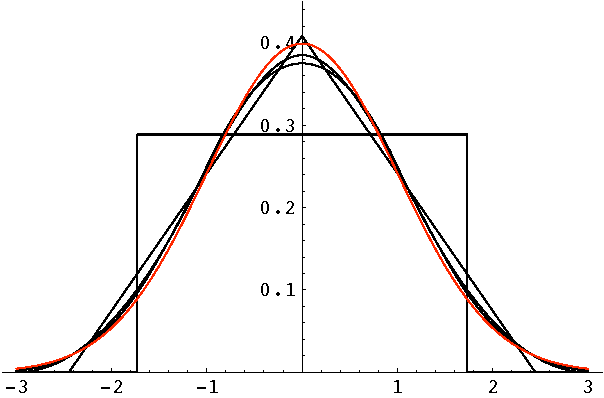
\includegraphics[width=0.8\hsize]{graphics/zgws}
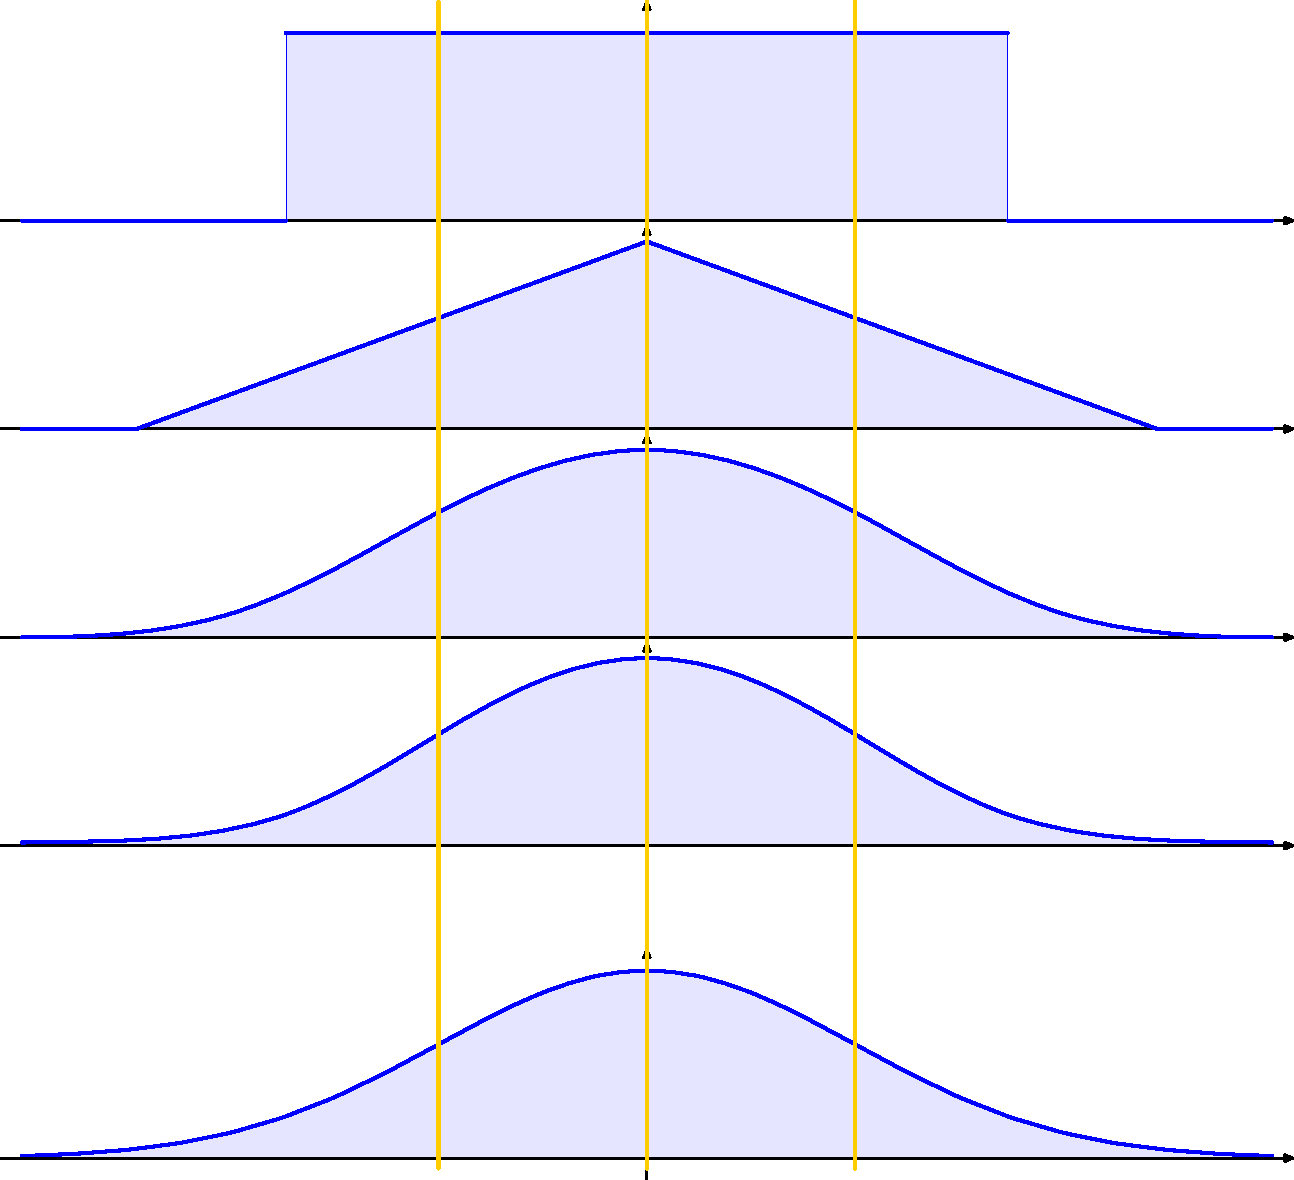
\includegraphics[width=\hsize]{images/verteilungsfunktion-10}
\end{center}
\caption{Zum zentralen Grenzwertsatz: die Wahrscheinlichkeitsdichte
der standardisierten Summe von bis zu vier 
gleichverteilten Zufallsvariablen (oben)
konvergiert gegen die Standardnormalverteilung (unten).\label{zgws}}
\end{figure}

Der zentrale Grenzwertsatz besagt nun, dass die Verteilungsfunktionen
von $S_n$ gegen die Verteilungsfunktion einer Normalverteilung
konvergieren\footnote{Wie genau diese Konvergenz gemeint ist, wird
im Laufe der Berechnung klar werden.}.
In den folgenden Abschnitten
versuchen wir, die Verteilungsfunktion von $S_n$ und insbesondere
ihren Grenzwert zu berechnen.
Die Abbildung \ref{zgws} illustriert
dies: dort wird die Wahrscheinlichkeitsdichte der standardisierten
Summe von bis zu vier im
Intervall $[-\sqrt{3},\sqrt{3}]$ gleichverteilte Zufallsvariablen dargestellt,
und mit der Standardnormalverteilung verglichen.

Wir betrachten als technisches Hilfsmittel für die Berechnung
die folgende Funktion:
\index{momenterzeugende Funktion}
\begin{definition} Ist $X$ eine Zufallsvariable, dann heisst die Funktion
\[
M_X(t)=t\mapsto E(e^{tX})=\sum_{k=0}^n\frac{t^k}{k!}E(X^k).
\]
die momenterzeugende Funktion von $X$
\end{definition}
Wir nehmen im folgenden
an, dass diese Funktion existiert\footnote{Für alle in diesem Kapitel
untersuchten Verteilungen trifft dies zu, es gibt aber auch Verteilungen,
für die die momenterzeugende Funktion nicht existiert, für die der
zentrale Grenzwertsatz aber trotzdem gilt.}.
Für die momenterzeugende
Funktion gilt die folgende Rechenregeln
\begin{align*}
M_{X+Y}(t)&=M_X(t)M_Y(t)\\
M_{\lambda X}(t)&=M_X(\lambda t)
\end{align*}

Wenn $\varphi$ die Dichtefunktion zur Zufallsvariable $X$ ist, dann
kann die momenterzeugende Funktion wie folgt berechnet werden:
\[
M_X(t)=E(e^{tX})=\int_{-\infty}^\infty e^{tx}\varphi(x)\,dx,
\]
die momenterzeugende Funktion ist also nichts anderes als eine
zweiseitige Laplacetransformierte von $\varphi$:
\[
M_X(t)={\cal L}\varphi(-t),
\]
insbesondere lässt sich in vielen Fällen aus der Laplacetransformierten
die ursprüngliche Funktion wieder bestimmen.
Der Plan ist daher der folgende:
\begin{enumerate}
\item Bestimme einen Näherungsausdruck für $M_{X_i}(t)$.
\item Bestimme einen Näherungsausdruck für $M_{S_n}(t)$.
\item Berechne den Grenzwert von $M_{S_n}(t)$ für $n\to\infty$.
\item Finde eine Verteilung, welche die gleiche Laplacetransformation
hat.
\end{enumerate}

{\parindent0pt\bf 1.~Schritt: Näherung für $M_{X_i}(t)$.} 
\index{Taylorreihe}
Aus der Taylorentwicklung von $e^{tX}$ folgt
\[
M_{X_i}(t)=1+E(X)t+\operatorname{var}(X)\frac{t^2}{2!}+R_i(t)t^2
=1+\frac{t^2}{2!}+R_i(t)t^2.
\]
Dabei ist das Restglied $R_i(t)$ so beschaffen, dass
$R_i(t)\to 0$ wenn $t\to 0$.

\medskip
{\parindent0pt\bf 2.~Schritt: Berechnung von $M_{S_n}(t)$.}
Aus den beiden Rechenregeln für die momenterzeugende Funktion folgt
jetzt zunächst für die Summe der Zufallsvariablen
\[
M_{X_1+\dots+X_n}(t)=M_{X_1}(t)\dotsm M_{X_n}(t),
\]
und anschliessen für das Produkt mit $\frac1{\sqrt{n}}$
\[
M_{S_n}(t)=M_{X_1}(t/\sqrt{n})\dotsm M_{X_n}(t/\sqrt{n}).
\]
Durch Einsetzen der Näherung aus dem ersten Schritt ergibt sich
\[
M_{S_n}(t)
=\prod_{i=1}^n\biggl(1+\frac{t^2}{2n}+R_i\biggl(\frac{t}{\sqrt{n}}\biggl)\frac{t^2}{n}\biggr)
=\biggl(1+\frac{t^2}{2n}+Q_n\biggl(\frac{t}{\sqrt{n}}\biggr)\frac{t^2}{n}\biggr)^n,
\]
wobei $Q_n(t)$ eine neue Funktion ist.
Diese kann durch
\[
Q_n(t/\sqrt{n})=\root{n}\of{M_{S_n}(t)}-1-\frac{t^2}{2n}
\]
ermittelt werden, und hat immer noch die Eigenschaft,
$\lim_{t\to0}Q_n(t)=0$.
Im einfachsten Fall, wenn die Zufallsvariablen
identisch verteilt sind, sind alle Funktionen $R_i$ gleich, und damit
auch alle $Q_n$.

\medskip
{\parindent0pt\bf 3.~Schritt: Grenzwert für $n\to\infty$.}
Für den Grenzübergang $n\to\infty$ beachten wir nun, schreiben wir
$M_{S_n}(t)$ mit Hilfe von
$x_n=\frac{t^2}2+Q_n(t)$
um als
\[
M_{S_n}(t)=\biggl(1+\frac{x_n}n\biggr)^n.
\]
Nun ist bereits aus der Analysis bekannt, dass
\[
\lim_{n\to\infty}\biggl(1+\frac{x}{n}\biggr)^n=e^x,
\]
es gilt aber auch in verallgemeinerter Form:
\[
\biggl(1+\frac{x_n}{n}\biggr)^n\to e^x\quad\text{falls}\quad x_n\to x.
\]
Da in unserem Fall $x_n\to \frac{t^2}2$, erhalten wir
\[
\lim_{n\to\infty}M_{S_n}(t)=e^{\frac{t^2}{2}}.
\]

\medskip
{\parindent0pt\bf 4.~Schritt: Die Grenzverteilung.}
Der gefundene Grenzwert soll die momenterzeugende Funktion einer
Verteilung sein, und wir erwarten, dass sie ebenfalls eine
momenterzeugende Funktion hat.
Da die momenterzeugende Funktion
nichts anderes als eine Laplacetransformation ist, können wir
den Eindeutigkeitssatz für die Laplacetransformation anwenden,
welcher besagt, dass zwei Funktionen, welche die gleiche zweiseitige
Laplacetransformierte haben, fast überall gleich sein.

Wir rechnen nach, dass $e^{\frac{t^2}2}$ die momenterzeugende Funktion
der Standardnormalverteilung ist.
Wir berechnen
dazu die Momente der Normalverteilung $\frac1{\sqrt{2\pi}}e^{-\frac{x^2}2}$
\begin{align*}
\int_{-\infty}^\infty e^{-\frac{x^2}2}x^{2k+1}\,dx&=0\\
\int_{-\infty}^\infty e^{-\frac{x^2}2}x^{2k}\,dx
&=
\biggl[\frac{x^{2k+1}}{2k+1}e^{-\frac{x^2}2}\biggr]_{-\infty}^\infty
+\frac1{(2k+1)}\int_{-\infty}^\infty x^{2k+2}e^{-\frac{x^2}2}\,dx\\
&=
\frac1{(2k+1)}\int_{-\infty}^\infty x^{2k+2}e^{-\frac{x^2}2}\,dx.
\end{align*}
Insbesondere kann man das $2k+2$-te Moment mit Hilfe einer
Rekursionsformel aus dem $2k$-ten Moment berechnen:
\[
E(X^{2k+2})=(2k+1)E(X^{2k}).
\]
Das $2k$-te Moment ist die Varianz, also $E(X^2)=1$.
Damit kann
man die momenterzeugende Funktion von $e^{-\frac{x^2}2}$ aufschreiben:
\begin{align*}
M(t)
&=
1+\frac{t^2}{2!} +\frac{t^4}{4!}3 +\frac{t^6}{6!}3\cdot5 +\frac{t^8}{8!}3\cdot5\cdot7+\dots\\
&=
1+\frac{t^2}{1!\cdot 2^1} +\frac{t^4}{2! \cdot 2^2} +\frac{t^6}{3!\cdot 2^3}
+\frac{t^8}{4!\cdot 2^4}\\
&=
1+(t^2/2) +\frac{(t^2/2)^2}{2!} +\frac{(t^2/2)^3}{3!}
+\frac{(t^2/2)^4}{4!}\\
&=e^{\frac{t^2}2}.
\end{align*}
Mit anderen Worten, die momenterzeugende Funktion der Normalverteilung
stimmt überein mit der momenterzeugenden Funktion der Grenzverteilung.
Schreiben wir $\varphi_n$ für die Dichtefunktion für $S_n$ und $F_n$
für die Verteilungsfunktion, dann gilt daher
nach allgemeinen Sätzen über die Laplacetransformation
\[
\lim_{n\to\infty}\varphi_n(x)=\frac1{\sqrt{2\pi}}e^{-\frac{x^2}2}
\quad\text{fast überall}
\]
und für die Verteilungsfunktion
\[
\lim_{n\to\infty}F_n(x)=\frac1{\sqrt{2\pi}}\int_{-\infty}^xe^{-\frac{t^2}2}\,dt.
\]
Insgesamt haben wir damit den folgenden Satz bewiesen:
\begin{satz}[Zentraler Grenzwertsatz]
\label{satz-zentraler-grenzwertsatz}
Sind $(X_i)_{1\le i}$ unabhängige Zufallsvariablen mit
Erwartungswert $E(X_i)=0$ und Varianz $\operatorname{var}(X_i)=1$
für alle $i\ge 1$.
Dann ist
\[
S_n=\frac1{\sqrt{n}}\sum_{i=1}^nX_i=\frac1{\sqrt{n}}(X_1+\dots+X_n)
\]
eine Folge von Zufallsvariablen, die ebenfalls Erwartungswert $E(S_n)=0$
und Varianz $\operatorname{var}(S_n)=1$ haben.
Falls die Zufallsvariablen
$X_i$
für alle $i$ eine momenterzeugende Funktion haben, hat auch $S_n$
für alle $n$ eine momenterzeugende Funktion, ausserdem konvergiert
die Verteilungsfunktion $F_n$ von $S_n$ gegen die Verteilungsfunktion der
Standardnormalverteilung
\[
\lim_{n\to\infty}F_n(x)=\frac1{\sqrt{2\pi}}\int_{-\infty}^xe^{-\frac{t^2}2}\,dt.
\]
Haben die $X_i$ ausserdem eine Wahrscheinlichkeitsdichte,
dann hat auch $S_n$
die Wahrscheinlichkeitsdichte $\varphi_n$, welche fast überall gegen die
Wahrscheinlichkeitsdichte der Standardnormalverteilung 
konvergiert:
\[
\lim_{n\to\infty}\varphi_n(x)=\frac1{\sqrt{2\pi}}e^{-\frac{x^2}2}.
\]
\end{satz}
